\chapter{Synthèse Bibliographique}

\section{Business Intelligence}
	\subsection{Introduction}
  		\paragraph{}
  		Dans le monde les grandes entreprises dans leurs activités journalières produisent une quantité importante de données qui a long terme devient en quantité astronomiques. Le besoin d’exploiter ces données a des fin de pilotage des entreprises a fait naitre le Business Intelligence encore appelé Intelligence Economique ou encore Informatique décisionnel qui permet d’étudier l’environnement de l’entreprise aux moyens des données qu’elle possède. Les données étant en grande quantité, il faut le nettoyer, les structures avant de les stocker dans ce qu’on a appelé Data Warehouse (Entrepôt de données en français).
  
  		\paragraph{}
  Le concept de Data Warehouse, tel que connu aujourd’hui, est apparu pour la première  fois en 1980 ; l’idée consistait alors à réaliser une base de données destinée exclusivement au processus décisionnel. Les nouveaux besoins de l’entreprise, les quantités importantes de données produites par les systèmes opérationnels et l’apparition des technologies aptes à sa mise en œuvre ont contribué à l’apparition du concept « Data Warehouse » comme support aux systèmes décisionnels.
  
  
	\subsection{Les systèmes décisionnels}
  		\paragraph{}
  L’entrepôt de données est au centre du système décisionnel et sa raison d’être est la mise en place de ces systèmes décisionnels. Nous allons ici rappeler quelques définitions qui serviront ont mieux expliqué la suite.
  \paragraph{}
  Selon Jean-Louis Le Moigne,  « Le système d’information est l’ensemble des méthodes et moyens de recueil de contrôle et de distribution des informations nécessaires à l’exercice de l’activité en tout point de l’organisation. Il a pour fonction de produire et de mémoriser les informations, de l’activité du système opérant (système opérationnel), puis de les mettre à disposition du système de décision (système de pilotage) » [Le Moigne 1977].
  \paragraph{}
  Selon Wikipédia, « L’informatique décisionnelle est l'informatique à l'usage des décideurs et des dirigeants    d'entreprises ».
  \paragraph{}
  De ces définition on retient que le système opérationnel et le système décisionnel sont des parties du                  système d’information. 
 


\begin{center}
	\begin{longtable}{|p{0.15\textwidth}|p{0.35\textwidth}|p{0.4\textwidth}|}
		\caption{Résume des différences entre le Transactionel et décisionnel.} 
		\label{Transactionel vs descisionel}
		\\
		
		
		\hline 
		\textbf{Critere} & 
		\textbf{Transact} &
		\textbf{discisionel}
		\\
		
		
		\endfirsthead
		\caption[]{Résume des différences entre le Transactionel et décisionnel (suite)} 
		\\
		\hline 
		\textbf{Différence} & 
		\textbf{Transactionel} &
		\textbf{déscisionel}
		\\
		\hline
		\endhead
		\hline
		\endfoot
		\hline
		
		
		\hline
		par les données &  
		
		\begin{description}
		 \item Orienté applications
		 \item Situation instantanée
		 \item Donnée détaillées et codées non redondantes
		 \item Données changeantes constamment
		 \end{description} &
		 
		 \begin{description}
		 \item Orienté thèmes et sujets
		 \item Situation historique
		 \item Informations agrégées cohérentes souvent avec redondance
		 \item Informations stables et synchronisées dans le temps
		 \end{description}
		\\ 
		
		\hline
		L’usage &  
		\begin{description}
		 \item Assure l’activité au quotidien
		 \item Pour les opérationnels
		 \item Mises à jour et requêtes simples
		 \item Temps de réponse immédiats
		 \end{description} &
		\begin{description}
		 \item Permet l’analyse et la prise de décision
		 \item Pour les décideurs
		 \item Lecture unique et requêtes complexes transparentes
		 \item Temps de réponse moins critiques
		 \end{description}
		\\  
		
		\hline 
	\end{longtable} 
\end{center}

\paragraph{}
	Ces différences font ressortir la nécessité de mettre en place un système répondant aux besoins décisionnels. Ce système n’est rien d’autre que le « Data Warehouse ».


\section{Le Data Warehouse}
 \subsection{Définition}
 Bill Inmon définit le Data Warehouse, dans son livre considéré comme étant la référence dans le domaine ``Building the Data Warehouse'' [Inmon, 2002] comme suit:
 
« Le Data Warehouse est une collection de données orientées sujet, intégrées, non volatiles et évolutives dans le temps, organisées pour le support d’un processus d’aide à la décision. »

Les paragraphes suivants illustrent les caractéristiques citées dans la définition d’Inmon.\\

\textbf{Orienté sujet}: le Data Warehouse est organisé autour des sujets majeurs de l’entreprise, contrairement à l’approche transactionnelle utilisée dans les systèmes opérationnels, qui sont conçus autour d’applications et de fonctions telles que : cartes bancaires, solvabilité client…, les Data Warehouse sont organisés autour de sujets majeurs de l’entreprise tels que : clientèle, ventes, produits…. Cette organisation affecte forcément la conception et l’implémentation des données contenues dans le Data Warehouse. Le contenu en données et en relations entre elles diffère aussi. Dans un système opérationnel, les données sont essentiellement destinées à satisfaire un processus fonctionnel et obéit à des règles de gestion, alors que celles d’un Data Warehouse sont destinées à un processus analytique.\\

\textbf{Intégrée }: le Data Warehouse va intégrer des données en provenance de différentes sources. Cela nécessite la gestion de toute incohérence.\\

\textbf{Evolutives dans le temps} : Dans un système décisionnel il est important de conserver les différentes valeurs d’une donnée, cela permet les comparaisons et le suivi de l’évolution des valeurs dans le temps, alors que dans un système opérationnel la valeur d’une donnée est simplement mise à jour. Dans un Data Warehouse chaque valeur est associée à un moment
« Every key structure in the data warehouse contains - implicitly or explicitly -an element of time » [Inmon, 2000].\\

\textbf{Non volatiles} : c’est ce qui est, en quelque sorte la conséquence de l’historisation décrite précédemment. Une donnée dans un environnement opérationnel peut être mise à jour ou supprimée, de telles opérations n’existent pas dans un environnement Data Warehouse. Organisées pour le support d’un processus d’aide à la décision : Les données du Data Warehouse sont organisées de manière à permettre l’exécution des processus d’aide à la décision (Reporting, Data Mining…).

 \subsection{Historique}
 	L’origine du concept « Data Warehouse » D.W (entrepôt de données en français) remonte aux années 80, durant lesquelles un intérêt croissant au système décisionnel a vu le jour, dû essentiellement à l’émergence des SGBD relationnel et la simplicité du modèle relationnel et la puissance offerte par le langage SQL, au début, le Data Warehouse n’était rien d’autre qu’une copie des données du système opérationnel prise de façon périodique, dédiée à un environnement de support à la prise de décision. Ainsi, les données étaient extraites du système opérationnel, stockées dans une nouvelle base de données «concept d’infocentre », le motif principal étant de répondre aux requêtes des décideurs sans pour autant altérer les performances des systèmes opérationnels. Le Data Warehouse, tel qu’on le connaît actuellement, n’est plus vu comme une copie ou un cumul de copies prises de façon périodique- des données du système opérationnel. Il est devenu une nouvelle source d’information, alimenté avec des données recueillies et consolidées des différentes sources internes et externes.
 
 \subsection{ARCHITECTURE D’UN DATA WAREHOUSE}
 
 	\begin{figure}[h]
	\begin{center}
		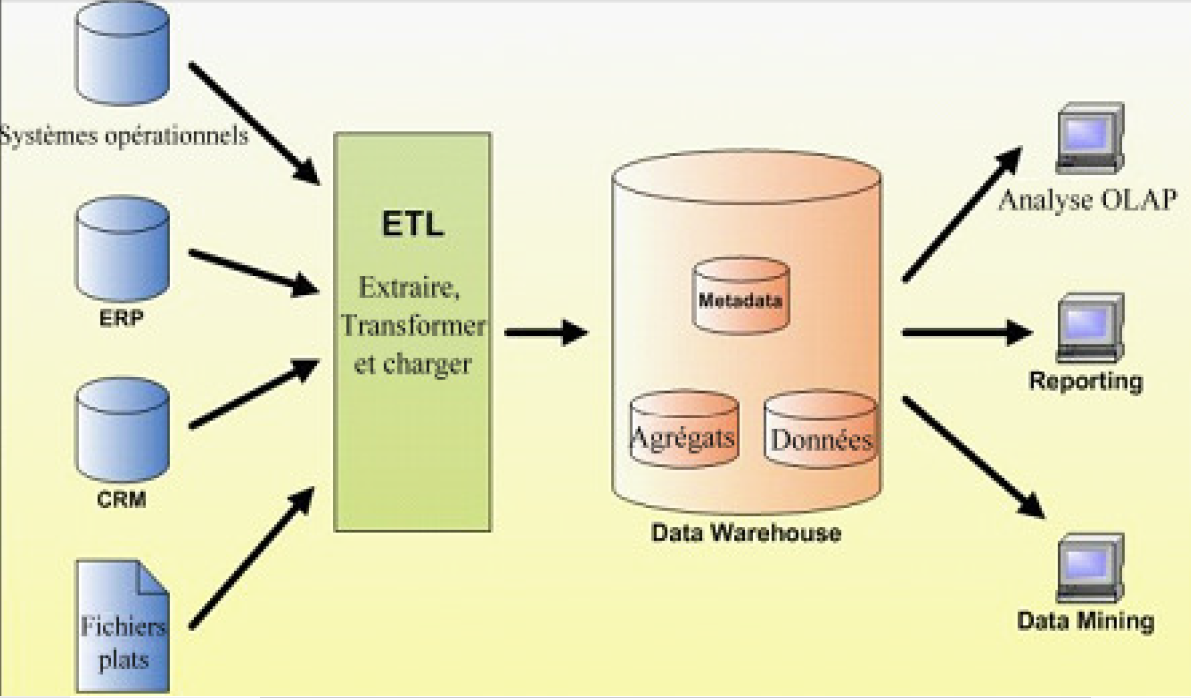
\includegraphics[scale=0.85]{images/DataWH.png}
		\caption{Architecture generale d'un data warehouse}
		\label{architecture-data-warehouse}
	\end{center}
\end{figure}

La figure ci-dessus Illustre la forme générale d’un data Warehouse que nous allons détailler dans les paragraphes suivants.

\textbf{Les Sources de données :} Dans la figure, les représentations de systèmes opérationnel, ERP, CRM et Fichiers plat font office de source de données et c’est d’elles qu’on puisse les données pour alimenter la machine décisionnelle.

\textbf{ETL (Extract, Transform, Load)}: C’est un ensemble de méthodes et d’outils qui servent a :\\
-	Extract : Extraire les données de sources hétérogènes\\
-	Transform : Transformation des données pour les mettre dans un format acceptable\\
-	Load : Charger les données dans le data warehouse\\

\textbf{Data Warehouse} : L’unité de stockage des données. Il est constitué de plusieurs éléments dont :\\ 
-	\textbf{Meta données} : ce sont les informations relatives à la structure des données, les méthodes d’agrégation et le lien entre les données opérationnelles et celles du Data Warehouse. Les métadonnées doivent renseigner sur :
 \begin{description}
 \item Le modèle de données,
 \item La structure des données telle qu’elle est vue par les développeurs,
 \item La structure des données telle qu’elle est vue par les utilisateurs,
 \item Les sources des données,
 \item Les transformations nécessaires,
 \item Suivi des alimentations,
 \end{description}
-	\textbf{Les Agrégats} (Données agrégées) : données agrégées à partir des données détaillées.\\

Les derniers éléments de la figure font partie de la phase d’exploitation du data warehouse et seront détaillés plus bas dans le document.


\section{Modélisation des données de l’entrepôt}

 \subsection{La modélisation dimensionnelle et ses concepts}
 	Les Data Warehouse sont destinés à la mise en place de systèmes décisionnels. Ces systèmes, devant répondre à des objectifs différents des systèmes transactionnels, ont fait ressortir très vite la nécessité de recourir à un modèle de données simplifié et aisément compréhensible. La modélisation dimensionnelle permet cela. Elle consiste à considérer un sujet d’analyse comme un cube à plusieurs dimensions, offrant des vues en tranches ou des analyses selon différents axes.
 	
 \begin{figure}[h]
	\begin{center}
		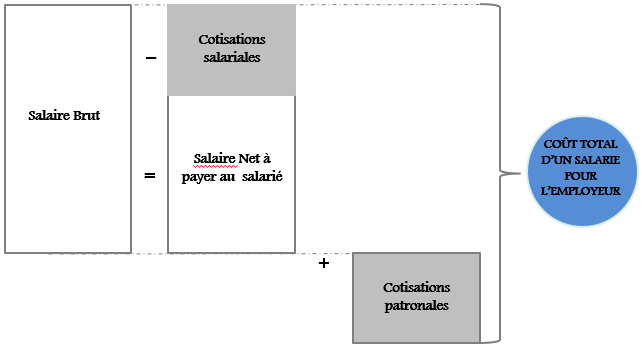
\includegraphics[scale=0.85]{images/remuneration.png}
		\caption{Considération d’un sujet d’analyse comme un cube à plusieurs dimensions.}
		\label{Cube-dimensionnel}
	\end{center}
\end{figure}
 
 
 \subsubsection{Le concept des Faits}
 	 Une table de faits est la table centrale d’un modèle dimensionnel, où les mesures de performances sont stockées. Une ligne d’une table de faits correspond à une mesure. Ces mesures sont généralement des valeurs numériques, additives ; cependant des mesures textuelles peuvent exister mais sont rares. Le concepteur doit faire son possible pour faire des mesures textuelles des dimensions, car elles peuvent êtres corrélées efficacement avec les autres attributs textuels de dimensions.
 
 \subsubsection{Le concept des Dimensions}
 
  Les tables de dimension sont les tables qui raccompagnent une table de faits, elles contiennent les descriptions textuelles de l’activité. Une table de dimension est constituée de nombreuses colonnes qui décrivent une ligne. C’est grâce à cette table que l’entrepôt de données est compréhensible et utilisable; elles permettent des analyses en tranches et en dés. Une dimension est généralement constituée : d’une clé artificielle, une clé naturelle et des attributs.
  
  
  
  
  
  
\begin{figure}[h]
	\begin{center}
		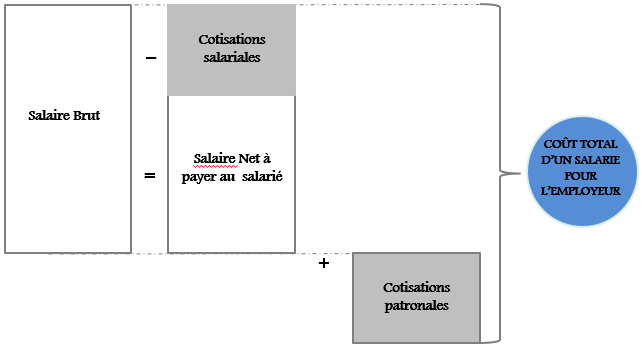
\includegraphics[scale=0.85]{images/remuneration.png}
		\caption{Schéma de synthèse sur le coût d'un salarié}
		\label{synthese-cout-salarie}
	\end{center}
\end{figure}

 











